\documentclass[a4paper, 11pt]{article}
\usepackage{fullpage}
\usepackage{url}
\usepackage{graphicx}
\usepackage{paralist}
\begin{document}
\title{[DRAFT]\\Customisation of Zombie Riot on\\i3D server \#04 [213.163.69.138:27015]}
\author{Dan ``Chimera'' Cassey}
\begin{figure}
\vspace{-20pt}
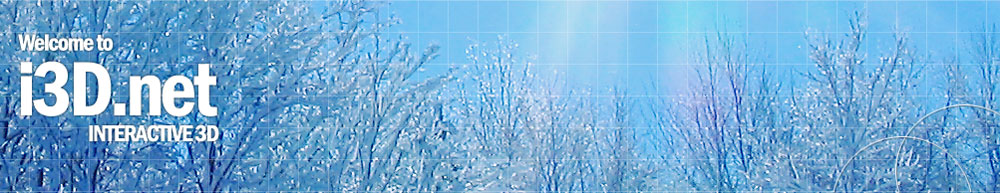
\includegraphics[width=\textwidth]{header-en.jpg}
\vspace{-60pt}
\end{figure}
\maketitle
\section{Introduction}
This document outlines the Specification and Design for the modification to the i3D Zombie Riot server as suggested by Rob.
\section{Night of the Dead server}
Rob's suggestions stem from a current server, located in the United States of America, called ``Night of the Dead''. The server runs Zombie Hell mod, the precursor to Zombie Riot, written for EventScripts. The server has been heavily customised, including a human class system, a currency system and player character customisation. Player customisation includes changing the character model, adding motion trails behind the player and adding player glow effects.
\section{Specification}
\begin{enumerate}
\item This project will be in the form of a plug-in for the SourceMod\cite{1} scripting platform, written in SourcePawn and using SQLite for local persistance.
\item This plug-in will be running on a Source Dedicated Server on Linux running Counter-Strike: Source
\item This plug-in will run in parallel with the Zombie Riot mod by Greyscale\cite{2}.
\item This plugin shall implement a human class system with the following classes:
\begin{description}
\item[Assault] Allows the player run faster.
\item[Sniper] Allows the player to cause more damage when using sniper rifles.
\item[Medic] Allows the player to heal team mates.
\item[Support] Gives the player 200\% more bullets per magazine for the M249 light machine gun.
\end{description}
These are the current classes on the Night of the Dead server. We may add further classes in the future as deemed necessary.
\item This plugin shall allow players to customise thier in-game character. This is to be implemented with a !shop menu where players can buy items for thier character and a credit system where players earn credits \begin{inparaenum}[\itshape a\upshape)]\item for in-game events such as joining the server, remaining on the server for a prolonged period of time and getting kills; or \item by selling previously purchased character modifications. \end{inparaenum}
\end{enumerate}
\section{Design}
\begin{thebibliography}{9}
\bibitem{1}
SourceMod: Half-Life 2 Scripting, \url{http://www.sourcemod.net/} [Online], accessed \today.
\bibitem{2}
Zombie Riot - Allied Modders, \url{http://forums.alliedmods.net/showthread.php?p=647040} [Online], accessed \today.
\end{thebibliography}
\vfill
\begin{figure}[h!]

\includegraphics[width=3cm]{Valve_logo.pdf}
\hfill

\includegraphics[width=3cm]{Counter-Strike_Source_logo.pdf}
\hfill

\includegraphics[width=3cm]{Source_engine_logo.pdf}
\end{figure}
Counter-Strike, the Counter-Strike logo, Source and the Source logo are trademarks and/or registered trademarks of Valve Corporation.
\end{document}